% This file was created with tikzplotlib v0.10.1.
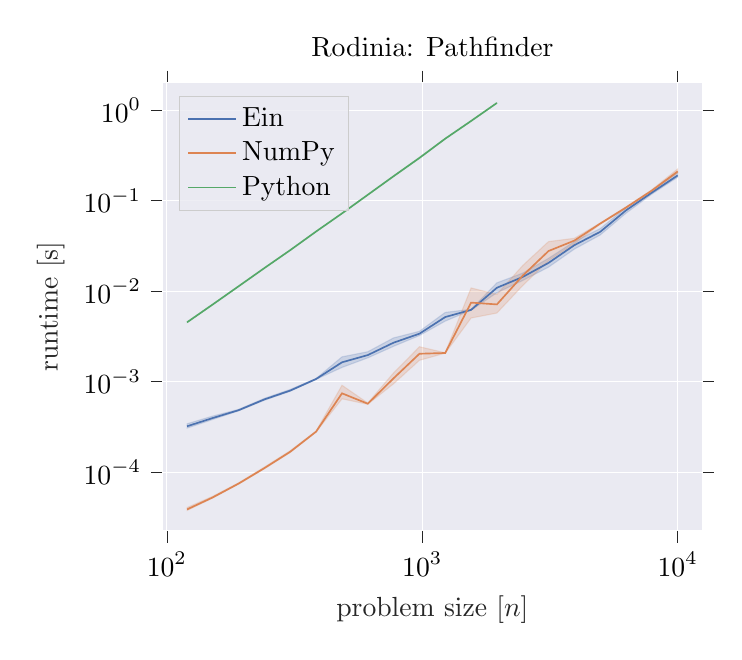
\begin{tikzpicture}

\definecolor{darkslategray38}{RGB}{38,38,38}
\definecolor{lavender234234242}{RGB}{234,234,242}
\definecolor{lightgray204}{RGB}{204,204,204}
\definecolor{mediumseagreen85168104}{RGB}{85,168,104}
\definecolor{peru22113282}{RGB}{221,132,82}
\definecolor{steelblue76114176}{RGB}{76,114,176}

\begin{axis}[
axis background/.style={fill=lavender234234242},
axis line style={white},
legend cell align={left},
legend style={
  fill opacity=0.8,
  draw opacity=1,
  text opacity=1,
  at={(0.03,0.97)},
  anchor=north west,
  draw=lightgray204,
  fill=lavender234234242
},
log basis x={10},
log basis y={10},
tick align=outside,
title={Rodinia: Pathfinder},
x grid style={white},
xlabel=\textcolor{darkslategray38}{problem size \(\displaystyle [n]\)},
xmajorgrids,
xmajorticks=true,
xmin=96.1922998493838, xmax=12475.0110131366,
xmode=log,
xtick style={color=darkslategray38},
xtick={1,10,100,1000,10000,100000,1000000},
xticklabels={
  \(\displaystyle {10^{0}}\),
  \(\displaystyle {10^{1}}\),
  \(\displaystyle {10^{2}}\),
  \(\displaystyle {10^{3}}\),
  \(\displaystyle {10^{4}}\),
  \(\displaystyle {10^{5}}\),
  \(\displaystyle {10^{6}}\)
},
y grid style={white},
ylabel=\textcolor{darkslategray38}{runtime \(\displaystyle [\mathrm{s}]\)},
ymajorgrids,
ymajorticks=true,
ymin=2.2418522596979e-05, ymax=2.02262511777973,
ymode=log,
ytick style={color=darkslategray38},
ytick={1e-06,1e-05,0.0001,0.001,0.01,0.1,1,10,100},
yticklabels={
  \(\displaystyle {10^{-6}}\),
  \(\displaystyle {10^{-5}}\),
  \(\displaystyle {10^{-4}}\),
  \(\displaystyle {10^{-3}}\),
  \(\displaystyle {10^{-2}}\),
  \(\displaystyle {10^{-1}}\),
  \(\displaystyle {10^{0}}\),
  \(\displaystyle {10^{1}}\),
  \(\displaystyle {10^{2}}\)
}
]
\path [draw=steelblue76114176, fill=steelblue76114176, opacity=0.2]
(axis cs:120,0.000341726930964796)
--(axis cs:120,0.000306472893898899)
--(axis cs:151,0.000380524324009457)
--(axis cs:191,0.000475164178642444)
--(axis cs:241,0.000622518288109859)
--(axis cs:304,0.000780791235338256)
--(axis cs:384,0.00105858095441363)
--(axis cs:485,0.0014339613285847)
--(axis cs:612,0.00182949863126851)
--(axis cs:772,0.00245332813254208)
--(axis cs:975,0.00322873239420005)
--(axis cs:1230,0.0046603400319691)
--(axis cs:1553,0.00614925598643822)
--(axis cs:1960,0.0095943368870212)
--(axis cs:2474,0.0131162009411673)
--(axis cs:3122,0.0184126407171061)
--(axis cs:3941,0.0291354026384579)
--(axis cs:4974,0.0417086751744864)
--(axis cs:6277,0.0726598048349842)
--(axis cs:7923,0.118049233426548)
--(axis cs:10000,0.1817131320034)
--(axis cs:10000,0.204999416671247)
--(axis cs:10000,0.204999416671247)
--(axis cs:7923,0.128127749075995)
--(axis cs:6277,0.083734567083649)
--(axis cs:4974,0.0490543335992334)
--(axis cs:3941,0.0353001864768157)
--(axis cs:3122,0.0230370064200542)
--(axis cs:2474,0.0158103541443779)
--(axis cs:1960,0.0123458300823404)
--(axis cs:1553,0.0063026045256629)
--(axis cs:1230,0.00581660559701049)
--(axis cs:975,0.00359588766476008)
--(axis cs:772,0.00303963665832271)
--(axis cs:612,0.00213747135527228)
--(axis cs:485,0.0018773853993298)
--(axis cs:384,0.00108018522152634)
--(axis cs:304,0.000818749898280657)
--(axis cs:241,0.000652531522373465)
--(axis cs:191,0.000493188765976811)
--(axis cs:151,0.000415084914093313)
--(axis cs:120,0.000341726930964796)
--cycle;

\path [draw=peru22113282, fill=peru22113282, opacity=0.2]
(axis cs:120,4.05292028394652e-05)
--(axis cs:120,3.76572221177818e-05)
--(axis cs:151,5.15489040017335e-05)
--(axis cs:191,7.37133692938077e-05)
--(axis cs:241,0.000108863147358759)
--(axis cs:304,0.00016458389057526)
--(axis cs:384,0.000277424925640168)
--(axis cs:485,0.000644754050045128)
--(axis cs:612,0.000561306121472983)
--(axis cs:772,0.000945457267077864)
--(axis cs:975,0.00171881254987961)
--(axis cs:1230,0.00206152069904944)
--(axis cs:1553,0.00504187347480254)
--(axis cs:1960,0.00572239232308683)
--(axis cs:2474,0.0115250413096875)
--(axis cs:3122,0.0217258990204398)
--(axis cs:3941,0.0334428679968257)
--(axis cs:4974,0.0548838507420711)
--(axis cs:6277,0.0824095292239567)
--(axis cs:7923,0.126775335965419)
--(axis cs:10000,0.201898616792484)
--(axis cs:10000,0.224101366947745)
--(axis cs:10000,0.224101366947745)
--(axis cs:7923,0.132007286081162)
--(axis cs:6277,0.0853363105666736)
--(axis cs:4974,0.0565887416299204)
--(axis cs:3941,0.0383505131565081)
--(axis cs:3122,0.03528248513181)
--(axis cs:2474,0.0192043702785523)
--(axis cs:1960,0.00920419509298448)
--(axis cs:1553,0.0108464514986388)
--(axis cs:1230,0.00208173524225237)
--(axis cs:975,0.0024281130370177)
--(axis cs:772,0.00124802802831195)
--(axis cs:612,0.00057954685688131)
--(axis cs:485,0.000910760384406102)
--(axis cs:384,0.000283834486956713)
--(axis cs:304,0.000172147029546981)
--(axis cs:241,0.00011356738586769)
--(axis cs:191,7.60678164252169e-05)
--(axis cs:151,5.38777557057058e-05)
--(axis cs:120,4.05292028394652e-05)
--cycle;

\path [draw=mediumseagreen85168104, fill=mediumseagreen85168104, opacity=0.2]
(axis cs:120,0.00455871063264353)
--(axis cs:120,0.00449157143116792)
--(axis cs:151,0.00705664282240553)
--(axis cs:191,0.0112666225017015)
--(axis cs:241,0.0179427403300778)
--(axis cs:304,0.0282595000777108)
--(axis cs:384,0.045413275318881)
--(axis cs:485,0.0720816022037464)
--(axis cs:612,0.115601016419376)
--(axis cs:772,0.18487746708988)
--(axis cs:975,0.293471200991418)
--(axis cs:1230,0.481217045161424)
--(axis cs:1553,0.755620449817535)
--(axis cs:1960,1.19882571494297)
--(axis cs:1960,1.2041320192535)
--(axis cs:1960,1.2041320192535)
--(axis cs:1553,0.766056252441126)
--(axis cs:1230,0.486687586993213)
--(axis cs:975,0.300764526207406)
--(axis cs:772,0.187704668997105)
--(axis cs:612,0.11655834188607)
--(axis cs:485,0.0725001043405431)
--(axis cs:384,0.0457697327409285)
--(axis cs:304,0.0284581307418256)
--(axis cs:241,0.0180423590589997)
--(axis cs:191,0.011370876864278)
--(axis cs:151,0.00713747732596371)
--(axis cs:120,0.00455871063264353)
--cycle;

\addplot [semithick, steelblue76114176]
table {%
120 0.000320914650365012
151 0.000395139447937254
191 0.000483020901447162
241 0.000635822951153386
304 0.000795981250121258
384 0.00106819585125777
485 0.0016338312496373
612 0.0019634500516986
772 0.00269066685068537
975 0.00338468330010073
1230 0.00516932915124926
1553 0.00620426465029595
1960 0.0108929021487711
2474 0.014341264700488
3122 0.0205118332502025
3941 0.0322111937006412
4974 0.0452253313495021
6277 0.0781504904600577
7923 0.122558375112324
10000 0.19009911116882
};
\addlegendentry{Ein}
\addplot [semithick, peru22113282]
table {%
120 3.86600244931162e-05
151 5.23924914005125e-05
191 7.46212748891676e-05
241 0.000110693301001573
304 0.000167543510974984
384 0.000279794247711953
485 0.000741863875427135
612 0.000569439187306788
772 0.00108637716541252
975 0.0020312529826725
1230 0.00207120530354192
1553 0.00746278985508761
1960 0.00712931676217431
2474 0.0148365315915019
3122 0.0277522884342686
3941 0.0361839926787512
4974 0.0557543046914908
6277 0.0839329969844282
7923 0.129218504613934
10000 0.210188051602755
};
\addlegendentry{NumPy}
\addplot [semithick, mediumseagreen85168104]
table {%
120 0.00452345369735408
151 0.00709796155077178
191 0.0113156319885714
241 0.0179928968837197
304 0.0283531498755143
384 0.0455828779890031
485 0.0722714566850368
612 0.116039105793265
772 0.186124559536344
975 0.296669488554691
1230 0.483990980228694
1553 0.759446551183138
1960 1.20162530253334
};
\addlegendentry{Python}
\end{axis}

\end{tikzpicture}
